\section{MQTT}
In questa sezione si passa alla descrizione del protocollo di rete MQTT ed al perchè si è scelto di utilizzare questa tecnologia.

\subsection{Descrizione}
Il protocollo MQTT (Message Queuing Telemetry Transport) è un protocollo di rete di tipo publish-subscribe, progettato per la trasmissione di messaggi tra dispositivi in ambienti caratterizzati da connessioni di rete con larghezza di banda limitata, latenza elevata, o affidabilità intermittente.

\noindent Le principali caratteristiche del protocollo MQTT includono:

\begin{itemize}
  \item \textbf{Efficienza nella larghezza di banda}: MQTT è progettato per minimizzare l'overhead di rete, il che lo rende particolarmente adatto per applicazioni in cui la larghezza di banda è limitata o costosa.
    
  \item \textbf{Affidabilità e livelli di qualità del servizio (QoS)}: MQTT offre tre livelli di QoS, che consentono di bilanciare la necessità di affidabilità con le risorse disponibili. I livelli QoS vanno da "almeno una volta" a "esattamente una volta", garantendo diversi gradi di consegna del messaggio in base ai requisiti dell'applicazione.
    
  \item \textbf{Supporto per la persistenza delle sessioni}: I client MQTT possono disconnettersi e riconnettersi senza perdere i messaggi inviati durante la disconnessione, grazie alla capacità del broker di mantenere lo stato delle sessioni e gestire i messaggi pendenti.

  \item \textbf{Sicurezza}: MQTT può essere configurato per utilizzare connessioni cifrate (SSL/TLS) e supporta l'autenticazione tramite username e password, garantendo la protezione dei dati scambiati e l'accesso controllato alle risorse.

  \item \textbf{Scalabilità}: La natura leggera e la flessibilità del modello publish-subscribe rendono MQTT altamente scalabile, consentendo di supportare un gran numero di dispositivi e applicazioni con un impatto minimo sulle risorse di rete.
\end{itemize}

\noindent Grazie a queste caratteristiche, MQTT è ampiamente utilizzato in una vasta gamma di applicazioni, tra cui la telemetria industriale, il monitoraggio ambientale, le smart cities, l'automazione domestica e i sistemi di gestione energetica, rappresentando una soluzione robusta ed efficiente per la comunicazione tra dispositivi eterogenei in contesti IoT.

\noindent All'interno del progetto per implementare lo stack MQTT si è avvalsi della libreria paho.mqtt.cpp\cite{paho_cpp}, una libreria open source fornita dalla eclipse foundation.

\subsection{Infrastruttura}
\noindent Il protocollo MQTT opera secondo un'architettura client-server, dove i client (dispositivi o applicazioni) si connettono a un server (broker) centrale che gestisce la distribuzione dei messaggi. I client che desiderano inviare dati pubblicano messaggi su specifici argomenti (topics), mentre i client interessati a ricevere quei dati si iscrivono (subscribe) agli stessi argomenti. Il broker, che agisce come intermediario, si occupa di ricevere i messaggi pubblicati e di inoltrarli a tutti i client iscritti agli argomenti corrispondenti.

\begin{figure}[H]
  \centering
  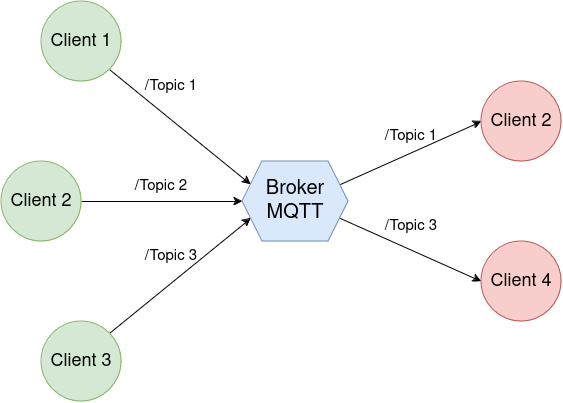
\includegraphics[width=0.8\textwidth]{figures/mqtt_structure.png}
  \caption{Struttura generica di un sistema di omunicazione basato su MQTT}
  \label{mqtt_structure}
\end{figure}

\noindent Nonostante questa numeclatura però, nel corso della presente tesi ci si riferirà al broker come "broker", mentre con il termine server ci si riferirà al calcolatore incaricato di ricevere i dati dal mezzo e a cui inviare i risultati (ovvero i messaggi di controllo).

\subsection{Formattazione messaggi}
I messaggi scambiati tramite protocollo MQTT non sono altro che stringhe di testo. È quindi necessario utilizzare una formattazione per il testo che ci renda possibile distinguere i vari campi di un messaggio ROS (la cui struttura è illustrata nella sezione precedente) che vogliamo inoltrare. Per questa motivazione si è deciso di avvalersi del formato JSON che si presta bene a questo impiego.

\noindent Per fare un esempio di seguito si illustra come un messaggio di odometria (illustrato nella sezione precedente)si presenterà in forma di testo JSON:

\lstinputlisting{samples/odometry.json}

\noindent Come si può vedere grazie a questa struttura è possibile rappresentare fedelmente i dati riportati dal messaggio ROS.

\subsection{Topic}
In MQTT, come in ROS, per dividere le varie tipologie di messaggi inoltrati si utilizzano i topic, questo in realtà è esattamente il motivo per cui si è deciso di utilizzare MQTT per il controllo remoto. Grazie infatti ad una semplice stuttura dati è possibile intercambiare tra le due tipologie di topic.

\noindent Ai fini del progetto è stata quindi sviluppata una classe chiamata \textit{topic\_manager} che semplifica la gestione di questi due tipi di dati. La classe comprende 4 semplici metodi, 2 che riguardano il get ed il set di topic ROS e 2 che riguardano il get e il set dei topic MQTT, ad ogni topic MQTT è associato uno ROS e viceversa, di seguito i 4 meotodi:

\lstinputlisting{samples/topic_manager.cpp}

\noindent È inoltre utile rendere nota la diversa struttura delle due tipologie di topic. Infatti, se per i topic ROS è utile utilizzare solo pochi identificatori, alle volte di una sola parola (eg. \textit{/drive\_parameters}, \textit{/scan}, \textit{/odometry}) dato che tutto il traffico ROS è presente solo all'interno del computer di bordo, per i topic MQTT è invece necessario utilizzare topic più lunghi, comprendenti diversi campi.

\noindent Per fare un esempio si può illustrare il topic utilizzato nell'odometria

\begin{center}
  /hipert/vehicle/rover\_1234/telemetry/odometry
\end{center}

\noindent Si elencano ora i diversi campi che compongono il topic

\begin{itemize}
  \item \textbf{/hipert}: È il campo che identifica il laboratorio che sta svolgendo la comunicazione, è utile in quanto se lo stesso broker MQTT è utilizzato da più laboratori abbiamo un filtro che ci permette di avere solo i dati rilevanti al nostro campo di interesse.
  \item \textbf{/vehicle}: Identifica il tipo di device osservato
  \item \textbf{/rover\_1234}: È l'effettiva stringa ID del topic, ci è utile per dare un identificatore univoco per il veicolo osservato, potremmo infatti anche avere più di un veicolo osservato e dobbiamo quindi sapere quale esattamente di questi si sta prendendo in considerazione.
  \item \textbf{/telemetry}: Identifica il tipo di dato preso in considerazione, infatti i dati potrebbero essere di tipo \textbf{telemetry}, \textbf{control} o eventualmente altro
  \item \textbf{/odometry}: Abbiamo infine l'esatto dato osservato, in questo caso, l'odometria del mezzo.
\end{itemize}
